\chapter{Methylation based plasmid binning using nanopore sequencing}
\label{chap:mdr}

\textbf{Portions of this chapter originally appeared in:} \\
Fan Y, Bergman Y, Workman R, Simner P, Timp W. Methylation based plasmid binning using nanopore sequencing. Unpublished.

\section{Abstract}
\label{sec:abstract}

Genomic analysis of microbial communities often involves reconstructing the full genomic complement of the community members after shotgun sequencing. However, contigs generated by metagenome assemblers typically only represent fragments of genomes and need to be further grouped together, a process known as ‘binning.’ Typical metagenomic binning methods rely primarily on signals from differential coverage and kmer spectra, but these can be confounded by mobile genetic elements, e.g. plasmids, since they can replicate independently of the chromosome and horizontally transfer between organisms. Current methods to resolve mobile genetic elements require more complex sample preparation or matched pairs of sequencing runs, making them more expensive and less accessible. A less used virtue of microbial systems is the “methylation fingerprint” where different bacteria have different methylation signatures as part of their restriction-modification (R-M) system. Using this, we tested the efficacy of metagenomic binning using methylation signal from a single ONT sequencing run. We find that we can correctly bin plasmids in a standard microbial community sample, and that we can identify a single plasmid appearing in different bacterial hosts. Furthermore, we applied this method to a clinical sample, and find that the results are largely consistent with binning methods based on proximity ligation.

\section{Introduction}
\label{sec:intro}

Metagenomics is the analysis of DNA extracted from whole microbial communities for resolving and linking the identities and functions of the community members(Strous et al. 2012). Common analysis steps involve assembling raw sequence reads into contigs, and clustering, or ‘binning’ them into metagenome assembled genomes (MAGs). Ideally, each MAG then represents the complete genetic complement of a community member, including any non-chromosomal DNA. From these MAGs, microbes can then be identified and genomic potential for functions such as metabolism, antimicrobial resistance, and pathogenicity can be inferred.

A number of computational tools have been developed for binning, the vast majority of which rely on k-mer spectra and coverage signals to differentiate between contigs originating from different organisms(Yue et al. 2020). While these methods work well for binning chromosomal contigs, they struggle to effectively bin plasmids(Beaulaurier et al. 2018). This is because plasmids are mobile elements which replicate independently from the bacterial chromosome, characteristics which confound the two key signals most binning methods rely upon.

Molecular biology methods like proximity ligation (Hi-C) have been used to successfully link MGEs and their hosts’ chromosomes(Burton et al. 2014). DNA inside of intact cells is crosslinked, then extracted and fragmented. Crosslinked fragments of DNA are then ligated together, and sequenced on a single read. Reads partially aligning to a chromosome and partially aligning to an MGE then provides evidence that the chromosome and MGE originated in a single cell. While this method has been shown to work well, it’s still somewhat limited by its need for two sequencing runs, intact bacterial samples, and longer, more labor intensive library preparation(Beyi et al. 2021).

More recently, binning methods that use DNA methylation detected by single molecule sequencing technologies have emerged(Beaulaurier et al. 2018; Tourancheau et al. 2021). These methods take advantage of the restriction-methylation systems in bacteria, which cause unique strains of bacteria to exhibit DNA methylation at potentially unique combinations of motifs. Importantly, these methylation patterns remain consistent across all of the chromosomes and plasmids of an individual strain, making them useful for associating any non-contiguous segments of DNA to each other. Methylation based binning with the Pacific Biosciences (Pacbio) single molecule real time (SMRT) sequencing platform relies on detecting pauses in the raw fluorescence signal (interpulse duration; IPD) to detect methylation. Currently available methods using the Oxford Nanopore Technologies (ONT) platform rely on comparing the raw electrical data generated by ONT sequencers in matched runs of methylated native DNA and completely unmethylated whole genome amplified(WGA) DNA(Tourancheau et al. 2021). Characteristic differences in electrical signal between the two runs can be used to locate and identify methylation. While this also works well, it requires two ONT sequencing runs and additional preparation work (WGA), again increasing the cost and limiting the scope of the method.

Here, we demonstrate a framework to perform metagenomic binning using methylation calls from a single single molecule sequencing run. Recent modifications to the BAM file specification have enabled base modification calls to be encoded from either PacBio or ONT data directly in the BAM file.  In our case, we used Megalodon to call methylation, a tool part of ONT’s stack of software, in conjunction with the all-context 5mC and 6mA modification model in Rerio, ONT’s suite of ‘research release’ basecalling models. On each metagenomic contig or reference sequence, we determine the methylation level at a combination of motifs, and use similarities in methylation levels at these motifs for binning. To assess binning performance, we examine a shared plasmid in a two-bacteria system, as well as a simple, synthetic microbial community. We then extend the method to a human microbiome sample, and compare to Hi-C results on the same sample.


\section{Results and Discussion}
\label{sec:results}

\subsection{Microbial Community Standard}
\label{sec:zymo}

To test the feasibility of associating plasmids to chromosomes, we used the ZymoBIOMICS Microbial Community Standard, which contains seven different species of bacteria and one yeast (Supp Table X_motifsummary). Among the bacteria in this sample, the E. coli strain contains a 110kb plasmid, and the S. aureus strain contains 3 plasmids with lengths 6.3kb, 2.2kb, and 2.9kb. As the identity of each species in the sample is known, we used their reference genomes to call methylation, and use these methylation signatures to bin plasmids with bacterial chromosomes.

To select the ‘barcode,’ or set of methylation motifs that would best differentiate between the species in the sample, we used the 6mA motifs and WGBS data published in McIntyre(McIntyre et al. 2017) et al. From the WGBS data, we identified the short (<8bp) 5mC motifs methylated in each species, and confirmed that these short motifs account for >99% of all 5mC methylation in these species (Supp Table 1). For both 6mA and 5mC motifs, only the short motifs of Type II and Type III MTases were included, since they comprise 85 of the 100 most frequently occurring methylation specificities listed in REBASE(Roberts et al. 2003). While excluding Type I motifs excludes the potential discriminatory power they provide, it also simplifies analysis by avoiding the long, ambiguous sections of the Type I bipartite motifs, e.g. EcoKI (AAC[N6]GTGC or GCAC[N6]GTT). Due to the absence of many motifs in the short S. aureus plasmids, we further narrowed the barcode to just GATC, CAGAG, CCWGG and CTKVAG (Supp Table X motifsummary). Despite this motif reduction, the two shortest S. aureus plasmids still did not have methylation calls for all four motifs (Supp Table X_zymo_meancov, Supp Table X zymo_motifcounts, Supp Fig X zymo_covhists), and were therefore excluded from further analysis. According to the WGBS and PacBio data(McIntyre et al. 2017) (Supp Table X_motif summary, Supp Table X_zymo_5mC), this four-motif barcode is theoretically sufficient to distinguish between all species except L. monocytogenes and P. aeruginosa, neither of which is methylated at any of the four motifs in the barcode. However, this reduction sufficiently preserves the methylation motifs specific to S. aureus and E. coli such that they are uniquely distinguishable from the other species in the sample, enabling us to correctly assign these plasmids to their hosts.

For each chromosome and plasmid, we constructed a methylation signature consisting of the average percent methylation at each of the four motifs in the barcode (Fig 1a). The percent methylation at each locus is calculated as the number of methylated calls out of the total number of calls made. Euclidean distance between these signatures was then used as a measure of similarity (Fig 1b). Notably, the methylation signatures closest to each of the plasmids correspond to the bacterial chromosomes of the species harboring each plasmid respectively. As expected, the distance between L. monocytogenes and P. aeruginosa are among the smallest between chromosomes because no motif included in the barcode differentiates between them. However, E. faecalis also groups closely with L. monocytogenes and P. aeruginosa. The only motif included in the barcode which separates E. faecalis from L. monocytogenes and P. aeruginosa is a 6mA motif (CTKV6mAG), and upon examination of the methylation signatures themselves, it becomes clear that this motif does not offer as much discriminatory power as the others (Fig 1a). In fact, removing this motif from the barcode does not appreciably change the distances between the chromosomes (Supp Fig 1).

To further explore, we implemented a barcode composed of only the relevant 5mC motifs (Supp Table 1). Due to the lack of CMT(5mC)GAKG occurrences on the S. aureus plasmid, we only classified the E. coli plasmid using this all-5mC barcode (Supp Fig 1). However, because the newly included CMT5mCGAKG is unique to P. aeruginosa, it is differentiable from L. monocytogenes and E. faecalis using this barcode. As expected, since the L. monocytogenes and E. faecalis strains in this sample do not exhibit any Type II 5mC methylation, these chromosomes remain close together in methylation space.

Methylation distance also can be calculated with tolerance for missing methylation values, where distances with missing values are scaled to as to be comparable to complete distances. By including all 5mC motifs in the barcode and forcing the classification of the S. aureus plasmid, P. aeruginosa again becomes differentiable from L. monocytogenes and E. faecalis (Supp Fig X). However, the distance between the S. aureus plasmid and chromosome also increases. While the shortest distances observed are still attributable to sequences with identical methylation, these distances are not as tight.

Notably, the methylation distances between the species in this community standard do not closely reflect their taxonomic lineages (Fig 1c). This indicates that methylome diversity is not determined by phylogeny, and suggests that methylation can potentially be used to distinguish between even closely related organisms.

\subsection{Two-bacteria System}
\label{sec:byard}

We then tested the efficacy of methylation signatures for accurately linking a single plasmid to different bacterial hosts. To do this, we used two bacteria, E. coli (strain DH5α) and S. aureus (strain RN4220), each containing an identical 10kb plasmid (pRW62). This plasmid contains an origin of replication for E. coli and a separate origin of replication for S. aureus so that it is replicated in both species. Both were cultured separately and sequenced separately on individual Flongle runs (Supp Table X_yields). With bisulfite sequencing data, we observed only two methylated loci in the entire genome of this strain of S. aureus, neither of which are in a known 5mC methylation context. In this strain of E. coli, all 5mC methylated loci occur in a C5mCWGG context.

Given the results of bisulfite analysis, we selected frequently recorded motifs in REBASE which include an adenine, as well as CCWGG. This resulted in a barcode of GATC, GANTC, CCWGG, CAGAG, CTKVAG, and GTWWAC. Because the methylated residues are not necessarily known for each motif, the base with the highest methylation percentage was chosen to represent each motif  locus. Again, the methylation signature of each sequence is represented by the average methylation percentages across all loci for each motif.

Using methylation signatures defined by these five motifs, we are able to distinguish the plasmid’s presence in E. coli from its presence in S. aureus (Fig 1d). However, when plasmid reads from both runs are mixed, combined and analyzed , the methylation signature places the mixed plasmid much closer to the E. coli signature than the S. aureus signature (Supp Fig 2a). This is partially because this plasmid has a much higher copy number in the E. coli data (Supp Table X_barnyard_runcov). When the E. coli plasmid reads are downsampled from 6000X coverage to 440X coverage to match the sequence coverage of the S. aureus reads before in silico mixing, the mixed plasmid moves away from the E. coli signature (Supp Fig 2b). Much of the remaining bias is accounted for by the high uncertainty of methylation calls at unmethylated loci (Supp Fig 3). Methylation callers such as Megalodon or nanopolish compute a probability that a base of a sequencing read is methylated(Simpson et al. 2017). This probability is then thresholded to call bases as either methylated, unmethylated, or uncertain. Though 5-methylcytosine in a CG context gives robust calls of either methylated or unmethylated(Simpson et al. 2017), non-CG 5-methylcytosine models are less robust and 6-methyladenine gives a smaller electrical signal shift, leading to more uncertain calls. Methylated motifs still present a high probability of methylation, but unmethylated motifs are less clear(supp Fig 3, supp Table X barnyard_modprobs). Unmethylated loci are less likely to contribute any methylation calls, suggesting that most calls made on the mixed plasmid originated from the E. coli data, the only organism with any confirmed methylation. To counteract this, we calculated methylation percentage as the ratio of methylated calls to the total coverage, instead of total methylation calls, at each locus. This way, the unmethylated calls do not play a role in determining the methylation signatures. With this adjustment, the mixed plasmid falls roughly equidistant between the E. coli and S. aureus signatures (Fig 1d). As methylation callers improve, we expect that this correction may not be necessary, because the values from methylation vs coverage and methylation vs called will converge.

Ensuring an equal mixture of plasmid reads is possible in simple systems where plasmid copy numbers are known or controlled, but it is not easily applicable in complex metagenomic contexts. While unnormalized contig-level methylation signatures can be effective for correctly identifying a single host, it is less reliable for identifying multiple hosts.
Clinical sample

Moving away from controlled samples, we wanted to examine the performance of methylation binning on a clinical stool sample, comparing the clustering results to a matched Hi-C library to provide a “ground truth”. From Illumina shotgun sequencing data, we assembled metagenomic contigs. These contigs were then binned using a matched Hi-C library, resulting in Hi-C bins, which are collections of Illumina contigs corresponding to the genetic complement of a member of the microbial community. We also sequenced the stool metagenome using the ONT platform, assembled metagenomic contigs using the ONT reads, and then polished these contigs using ONT read alignments (Supp Table X_asmstats). These polished metagenomic contigs represent segments of DNA found in the microbial community, but are not binned or otherwise grouped in any way. In order to group these contigs, we called methylation and used this methylation signal to bin the long-read contigs.

Because the relevant methylation motifs in this sample are unknown, we selected the most frequently occurring ones in REBASE, as recently used by(Tourancheau et al. 2021), then narrowed these down further to the 14 motifs that occur at least once in each contig on a sufficient number of contigs, preferentially keeping 5mC motifs  (Supp Table 2, Supp Table X motifs_considered). We calculated a methylation signature for each contig using the percent methylation at each motif, then clustered contigs using the Euclidean distance between signatures. Polished ONT contigs were then matched to Hi-C bins using whole genome alignment.

\subsection{Clinical Sample}
\label{sec:mdr}

Moving away from controlled samples, we wanted to examine the performance of methylation binning on a clinical stool sample, comparing the clustering results to a matched Hi-C library to provide a “ground truth”. From Illumina shotgun sequencing data, we assembled metagenomic contigs. These contigs were then binned using a matched Hi-C library, resulting in Hi-C bins, which are collections of Illumina contigs corresponding to the genetic complement of a member of the microbial community. We also sequenced the stool metagenome using the ONT platform, assembled metagenomic contigs using the ONT reads, and then polished these contigs using ONT read alignments (Supp Table X_asmstats). These polished metagenomic contigs represent segments of DNA found in the microbial community, but are not binned or otherwise grouped in any way. In order to group these contigs, we called methylation and used this methylation signal to bin the long-read contigs.

Because the relevant methylation motifs in this sample are unknown, we selected the most frequently occurring ones in REBASE, as recently used by(Tourancheau et al. 2021), then narrowed these down further to the 14 motifs that occur at least once in each contig on a sufficient number of contigs, preferentially keeping 5mC motifs  (Supp Table 2, Supp Table X motifs_considered). We calculated a methylation signature for each contig using the percent methylation at each motif, then clustered contigs using the Euclidean distance between signatures. Polished ONT contigs were then matched to Hi-C bins using whole genome alignment.

To assess the performance of this methylation based clustering compared to Hi-C, we show the ‘contamination’ and ‘completeness’ of clusters as defined by different height thresholds on the tree, where height corresponds to methylation-based Euclidean distance. Here, ‘contamination’ is the percentage of contigs not contained in a cluster with only other contigs of the same Hi-C bin, while ‘completeness’ is the percentage of contigs contained in the same cluster as the majority of contigs of its bin (Fig 2a). Similar to a receiver operating curve (ROC) for binary classifiers, an ideal clustering would have either 0%  contamination or 100% togetherness at all height thresholds, resulting in an AUC of 1. Unlike an ROC, a random classifier would not be represented by a diagonal line, but a decay-like function, according to simulated random clustering.

Moving to mobile elements, we found that contigs identified as plasmids belong to the same methylation distance clusters as Hi-C bins.  For all eight plasmid contigs with full barcode information,  the nearest contigs come from the same bin (Fig 2b,c). While these pairwise distance calculations can be done using a subset of motifs in the barcode if a plasmid contig does not contain all the motifs, the number of nearby contigs belonging to the same bin decreases as motifs are removed (Fig 2c).

Using PlasmidFinder, we identified which nanopore contigs were likely to be plasmids, and using Kraken2, we classified them taxonomically (Supp Table X plasmid_analysis). Of the nanopore contigs identified as plasmids, three were classified as K. pneumoniae sequences. These were an IncFIB(pQil) plasmid, an IncM2 plasmid, and a plasmid identified as both IncX3 and ColKP3. However, the IncM2 and the IncX3/ColKP3 plasmids align to a Hi-C bin that is predominantly composed of E. coli sequences (bin_3) (Supp Table X tigbin_species_kraken), suggesting that E. coli was the host organism for these plasmids in the original sample. Methylation distance corroborates this, as the nearest contigs to these two plasmid contigs are also both classified as E. coli sequences (Supp Table X plasmid_analysis). However, a ColKP3 sequence was detected in the Illumina contigs making up the K. pneumoniae Hi-C bin_5. While this could indicate a mis-assembly of the IncX3/ColKP3 nanopore contig, coverage profiles across each plasmid contig did not exhibit any stepwise or aberrant changes. Furthermore, the flye assembler indicates that the IncX3/ColKP3 contig is circular, suggesting that mis-assembly is unlikely, though not impossible. Without using orthogonal information from either Hi-C or methylation, correctly identifying the host of these plasmids as E. coli would not have been possible.

\section{Discussion}
\label{sec:discuss}



\section{Methods}
\label{sec:methods}

\subsection{Media and growth conditions}
\label{sec:methods}

For genomic extractions, a single colony of \textit{C. nivariensis} CBS9983, originally isolated from a blood culture of a Spanish woman \citep{Alcoba-Florez2005-xn}, was inoculated into synthetic complete (SC) medium supplemented with 2\% glucose and shaken overnight at 30°C in a glass culture tube. For RNA extractions, \textit{C. nivariensis} CBS9983 was grown to log phase in SC medium supplemented with 2\% glucose at 30°C in a glass culture tube.

\subsection{DNA isolation and sequencing}
\label{sec:methods}

DNA was extracted from liquid culture using the Zymo Fungal/Bacterial DNA MiniPrep Kit according to manufacturer specifications. Two ONT sequencing libraries were prepared from the extracted DNA using the ONT rapid barcoding sequencing kit (SQK-RBK004), and each was sequenced on a separate MinION flowcell (R9.4). Two Illumina libraries were prepared with the Nextera Flex Library Prep Kit, each using 400 ng of extracted DNA. Both Illumina libraries were then sequenced on a single iSeq 100 run.

\subsection{RNA isolation and sequencing}
\label{sec:methods}

RNA was extracted from liquid culture using the Zymo Fungal/Bacterial RNA MiniPrep Kit. Using the NEBNext Poly(A) mRNA Magnetic Isolation Module, polyA tailed mRNA was isolated from the total RNA. Two ONT direct RNA sequencing libraries were prepared and sequenced on separate MinION flowcells, each using ∼200 ng of polyA selected RNA and the SQK-RNA002 sequencing kit. With the NEBNext Ultra II RNA First-Strand Synthesis Module and the NEBNext Ultra II Non-Directional RNA Second Strand Synthesis Module, cDNA was prepared from the isolated mRNA. Two individual Illumina libraries were then prepared with the Nextera Flex Library Prep Kit, each using 400 ng of cDNA. Both library replicates were then sequenced on a single iSeq 100 run, generating 2 × 150 paired-end reads.

\subsection{Genome assembly}
\label{sec:methods}

Nanopore data were basecalled using Guppy v3.2.4 on default settings. Reads greater than 3 kb long with an average basecalling quality score greater than 7 were assembled into 21 contigs using Canu v2.1 \citep{Koren2017-wf} on default settings with the genome size set to 11 m. Illumina DNA reads were trimmed for adapters and quality using Trimmomatic v0.39 \citep{Bolger2014-ax} using settings \texttt{LEADING:3 TRAILING:3 SLIDINGWINDOW:4:30 MINLEN:36}. The trimmed reads were then used to iteratively correct draft assembly using Freebayes v1.3.4-pre1 \citep{Garrison2012-iq} with alignments made by bwa mem v0.7.17-r1198-dirty \citep{Li2013-ec} using default settings. Changes were made at positions where both the alternative allele frequency was greater than 0.5 and the total number of alternate allele observations was greater than 5. We aligned and corrected the assembly iteratively for three rounds, after which further rounds of corrections made no changes.

Of our 21 corrected contigs, 5 were flagged as repeats by Canu and originally constructed from fewer than 180 nanopore reads. The remaining 16 contigs were constructed from over 1800 nanopore reads each. Because the five repetitive contigs were constructed from so few reads and were found to occur elsewhere in the assembly through Mummer v4.0.0rc1 \citep{Marcais2018-mm} and nanopore read alignment Minimap2 v2.17 \citep{Li2018-eq}, we excluded them from the final assembly. One 32-Kb contig was suggested to be circular by Canu, and therefore likely to be a mitochondrial sequence. To confirm, we aligned this contig to the complete mitochondrial genome of \textit{C. nivariensis} (NCBI: NC\_036379.1) using Mummer, and observed a 3662-bp sequence in the reference mitochondrial genome which appears at both ends of our 32-kb circular contig. Using the Mummer alignments ({\bf Figure \ref{fig:mito}}), we removed the extraneous 3662 bp from the end of our contig, resulting in a 28-kb mitochondrial genome, which we named “JHU\_Cniv\_v1\_mito.” Lastly, we remapped the ONT and Illumina reads back to the assembly, and found no bases with zero coverage, indicating that none of our contigs need to be further broken ({\bf Figure \ref{fig:covhist}}). Henceforth, we refer to this assembly as “JHU\_Cniv\_v1.”

\begin{kframe}
\begin{alltt}
\hlstd{what} \hlkwb{<-} \hlstr{"figure"}
\hlstd{figname} \hlkwb{<-} \hlstr{"mito"}
\hlstd{title} \hlkwb{<-} \hlstr{"Alignment of JHU\textbackslash{}\textbackslash{}_Cniv\textbackslash{}\textbackslash{}_v1 mitochrondrial contig and the \textbackslash{}\textbackslash{}textit\{C. nivariensis\} mitochondrial genome"}
\hlstd{desc} \hlkwb{<-} \hlstr{"Alignment of our 32Kb circular contig (x axis) with the completed mitochondrial genome of the \textbackslash{}\textbackslash{}textit\{C. nivariensis\} reference genome (y axis). The final 3662bp of this contig appears twice in the reference genome."}
\hlstd{shortname} \hlkwb{<-} \hlstr{"fig:mito"}
\hlstd{where} \hlkwb{<-} \hlstr{"[!ht]"}

\hlstd{figstr} \hlkwb{<-} \hlkwd{paste0}\hlstd{(}\hlstr{'\textbackslash{}\textbackslash{}begin\{'}\hlstd{, what ,}\hlstr{'\}'}\hlstd{, where ,}\hlstr{'
\textbackslash{}\textbackslash{}centering
\textbackslash{}\textbackslash{}includegraphics[width = 1\textbackslash{}\textbackslash{}linewidth,keepaspectratio]\{figure/'}\hlstd{, figname,} \hlstr{'.pdf\}
\textbackslash{}\textbackslash{}caption['}\hlstd{, title ,}\hlstr{']\{\{\textbackslash{}\textbackslash{}bf '}\hlstd{, title  ,}\hlstr{'.\} '}\hlstd{, desc ,}\hlstr{' \}
\textbackslash{}\textbackslash{}label\{'}\hlstd{, shortname ,}\hlstr{'\}
\textbackslash{}\textbackslash{}end\{'}\hlstd{, what ,}\hlstr{'\}
'}\hlstd{)}
\hlkwd{cat}\hlstd{(figstr)}
\end{alltt}
\end{kframe}\begin{figure}[!ht]
\centering
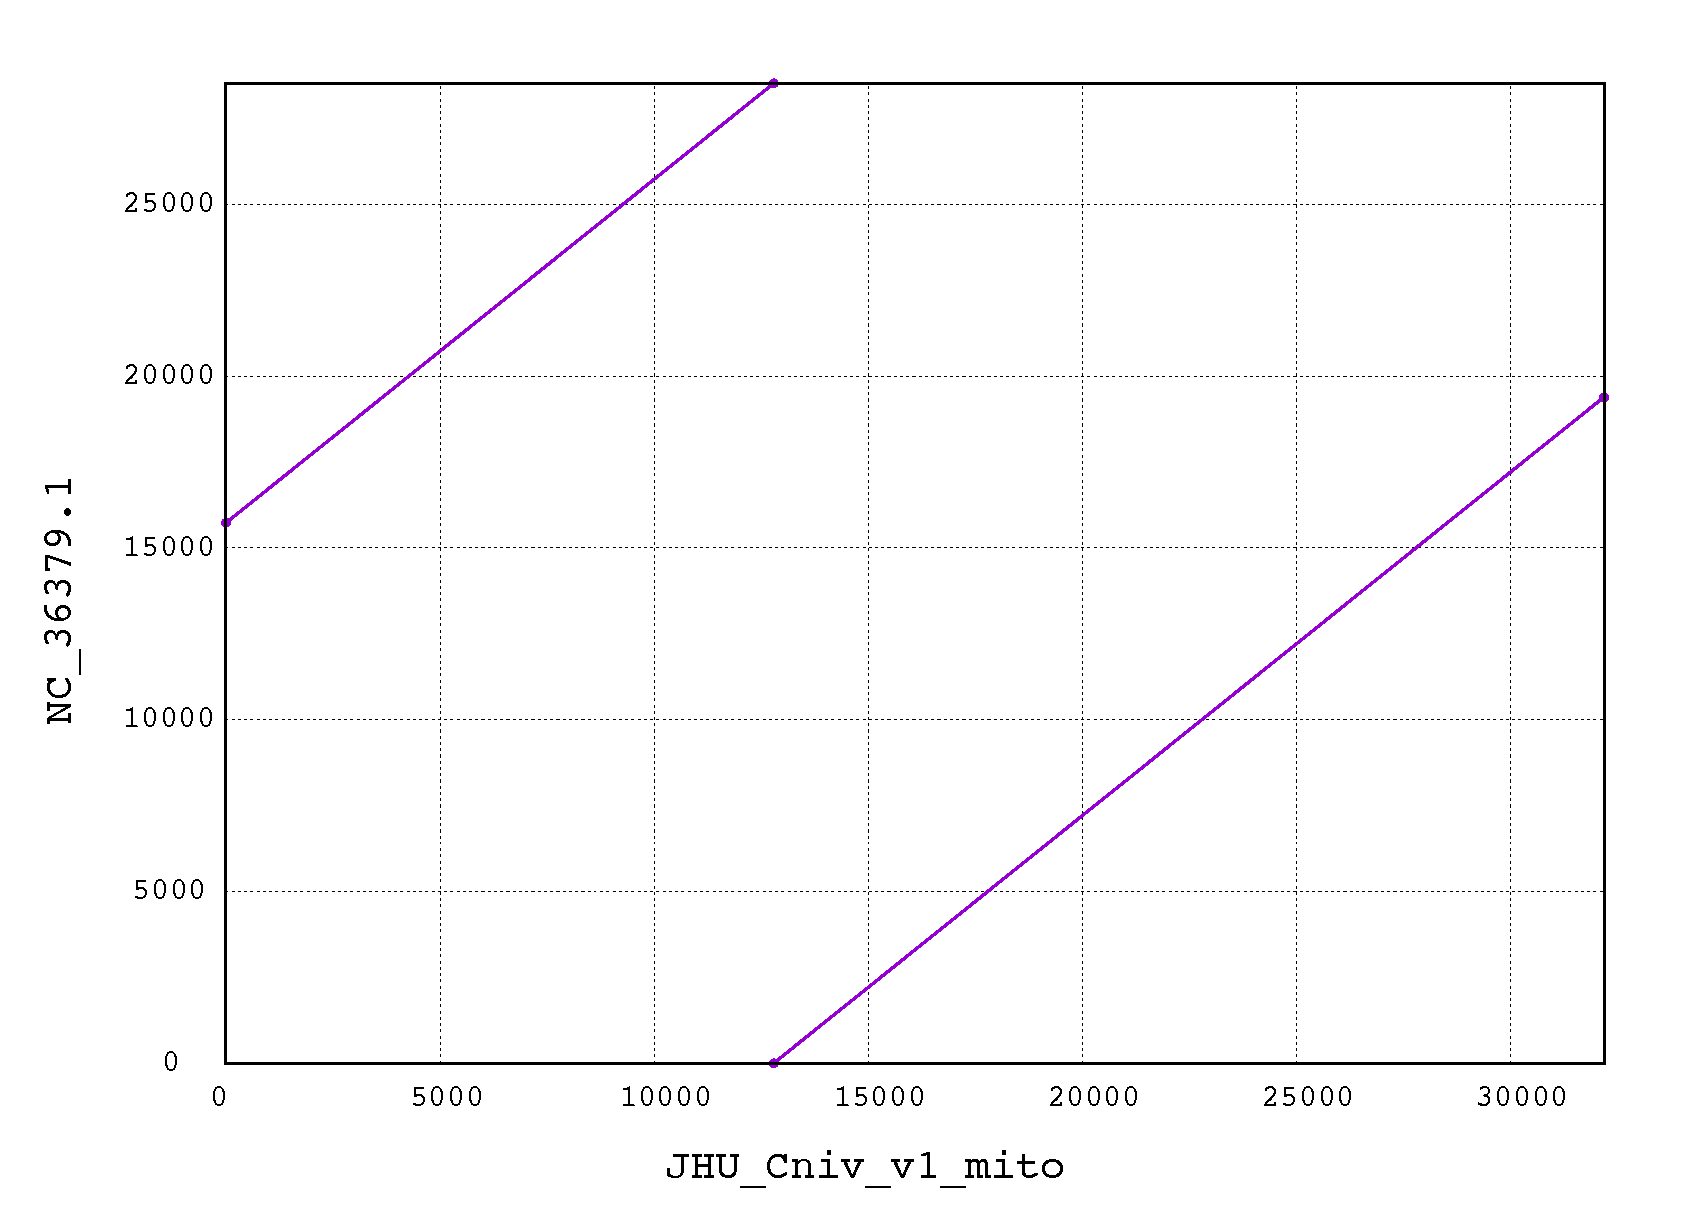
\includegraphics[width = 1\linewidth,keepaspectratio]{figure/mito.pdf}
\caption[Alignment of JHU\_Cniv\_v1 mitochrondrial contig and the \textit{C. nivariensis} mitochondrial genome]{{\bf Alignment of JHU\_Cniv\_v1 mitochrondrial contig and the \textit{C. nivariensis} mitochondrial genome.} Alignment of our 32Kb circular contig (x axis) with the completed mitochondrial genome of the \textit{C. nivariensis} reference genome (y axis). The final 3662bp of this contig appears twice in the reference genome. }
\label{fig:mito}
\end{figure}


\begin{kframe}
\begin{alltt}
\hlstd{what} \hlkwb{<-} \hlstr{"figure"}
\hlstd{figname} \hlkwb{<-} \hlstr{"covhist"}
\hlstd{title} \hlkwb{<-} \hlstr{"Coverage histograms"}
\hlstd{desc} \hlkwb{<-} \hlstr{"Histogram of coverage per base in our assembly by filtered (>3kb) ONT reads and trimmed Illumina reads."}
\hlstd{shortname} \hlkwb{<-} \hlstr{"fig:covhist"}
\hlstd{where} \hlkwb{<-} \hlstr{"[!ht]"}

\hlstd{figstr} \hlkwb{<-} \hlkwd{paste0}\hlstd{(}\hlstr{'\textbackslash{}\textbackslash{}begin\{'}\hlstd{, what ,}\hlstr{'\}'}\hlstd{, where ,}\hlstr{'
\textbackslash{}\textbackslash{}centering
\textbackslash{}\textbackslash{}includegraphics[width = 1\textbackslash{}\textbackslash{}linewidth,keepaspectratio]\{figure/'}\hlstd{, figname,} \hlstr{'.pdf\}
\textbackslash{}\textbackslash{}caption['}\hlstd{, title ,}\hlstr{']\{\{\textbackslash{}\textbackslash{}bf '}\hlstd{, title  ,}\hlstr{'.\} '}\hlstd{, desc ,}\hlstr{' \}
\textbackslash{}\textbackslash{}label\{'}\hlstd{, shortname ,}\hlstr{'\}
\textbackslash{}\textbackslash{}end\{'}\hlstd{, what ,}\hlstr{'\}
'}\hlstd{)}
\hlkwd{cat}\hlstd{(figstr)}
\end{alltt}
\end{kframe}\begin{figure}[!ht]
\centering
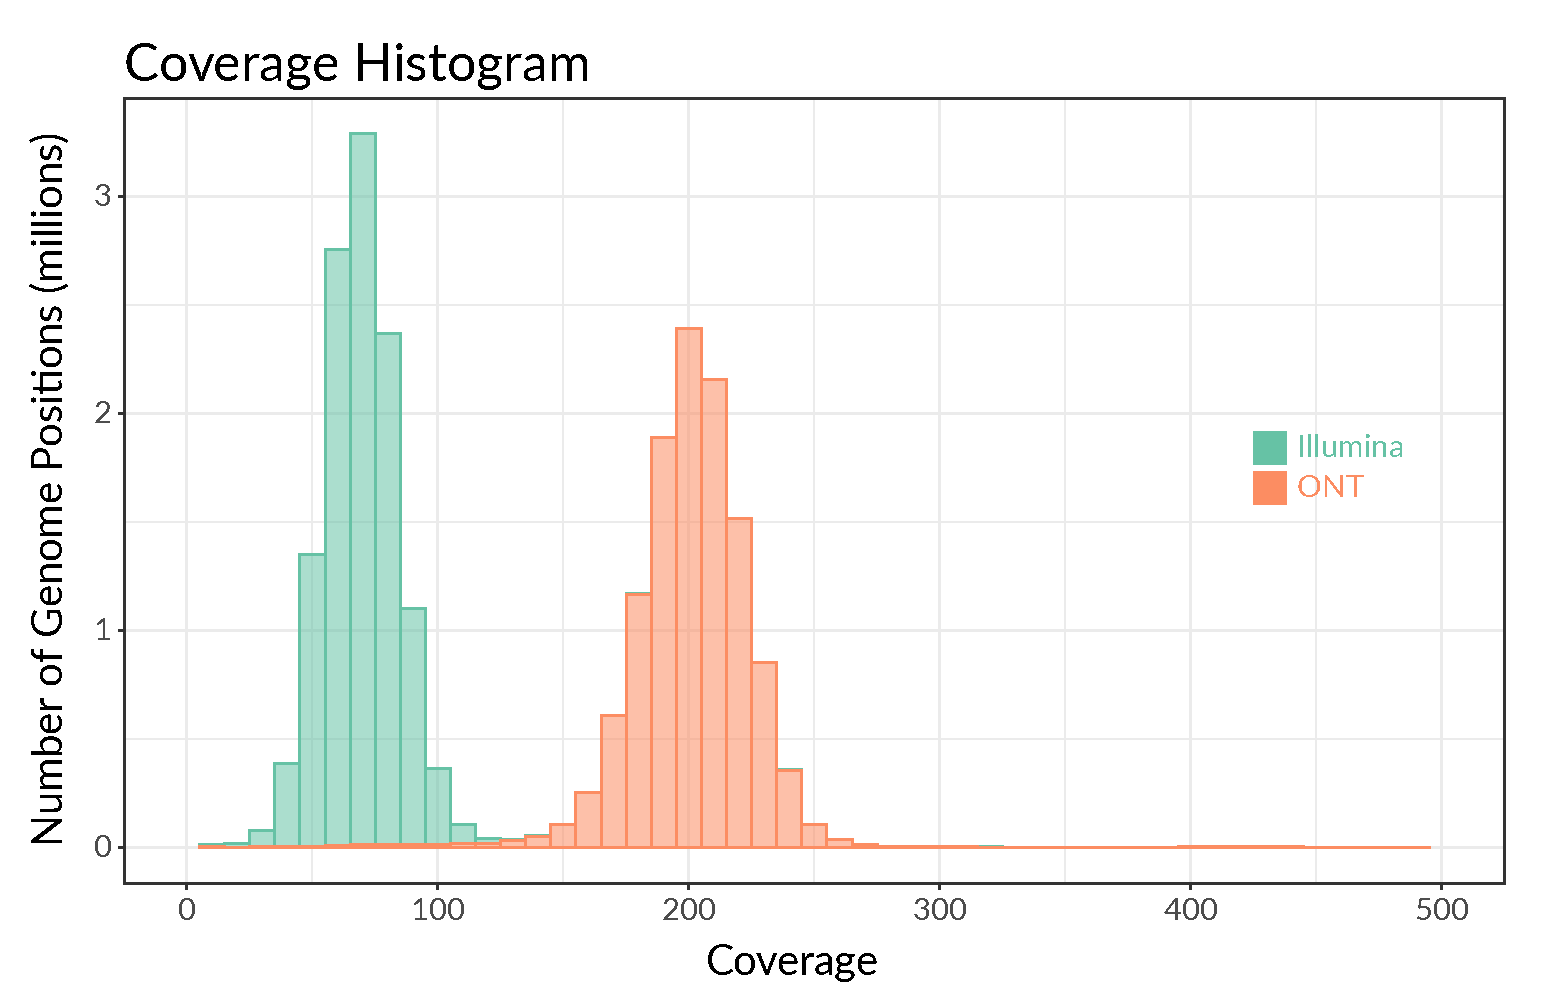
\includegraphics[width = 1\linewidth,keepaspectratio]{figure/covhist.pdf}
\caption[Coverage histograms]{{\bf Coverage histograms.} Histogram of coverage per base in our assembly by filtered (>3kb) ONT reads and trimmed Illumina reads. }
\label{fig:covhist}
\end{figure}


Repeat regions were identified by Tandem Repeats Finder v4.09 \citep{Benson1999-lr} with settings \citep{Xu2020-ta}: \texttt{match = 2, mismatch = 7, delta = 7, pm = 80, pi = 10, minscore = 50, maxperiod = 600}. Multimapping short reads were identified using bwa mem \citep{Li2013-ec} on default settings.

\subsection{Annotation}
\label{sec:methods}

Illumina RNA-seq reads were trimmed using Trimmomatic v0.39 \citep{Bolger2014-ax} in order to check for any remaining adapter sequences and to filter out reads with low base quality. HISAT2 v2.1.0 was used on default settings to align the trimmed cDNA reads to the assembly. The BRAKER v2.1.5 pipeline \citep{Hoff2019-rd} was then used to make gene predictions using these alignments. Currently, ONT dRNA compatibility with BRAKER is in development, and that data was thus not used for prediction. Instead, ONT dRNA reads were aligned to the genome assembly using Minimap2 on recommended settings for nanopore direct RNA reads (\texttt{-ax splice -uf -k14}). Transcripts were then assembled from the dRNA alignments using StringTie2 v2.1.5 \citep{Kovaka2019-lg} with the long read option (\texttt{-L}). Using Liftoff v1.5.0 \citep{Shumate2020-fo}, we lifted over the annotations from \textit{C. glabrata} (NCBI: GCF\_000002545.3), \textit{Saccharomyces cerevisiae} (NCBI: GCF\_000146045.2), \textit{Candida albicans} (NCBI: GCF\_000182965.3).

Starting with the BRAKER predictions, GffCompare v0.12.1 \citep{Pertea2020-lw} was used to add nonoverlapping annotations lifted from \textit{C. glabrata}, \textit{S. cerevisiae}, and \textit{C. albicans} in that order. Specifically, we add any annotation with class code “u” in the GffCompare .tmap outputs when comparing our list of genes with a list of potential genes to add, since these refer to intergenic regions devoid of any overlap or proximity to previous annotations. Finally, we compared and added nonredundant transcripts assembled by StringTie2 to the annotation using GffCompare.

\begin{kframe}
\begin{alltt}
\hlstd{what} \hlkwb{<-} \hlstr{"table"}
\hlstd{figname} \hlkwb{<-} \hlstr{"genecounttable"}
\hlstd{title} \hlkwb{<-} \hlstr{"Contributions from each annotation software"}
\hlstd{desc} \hlkwb{<-} \hlstr{"Number of genes and exons added by each software"}
\hlstd{shortname} \hlkwb{<-} \hlstr{"tab:genecounttable"}
\hlstd{where} \hlkwb{<-} \hlstr{"[!ht]"}

\hlstd{figstr} \hlkwb{<-} \hlkwd{paste0}\hlstd{(}\hlstr{'\textbackslash{}\textbackslash{}begin\{'}\hlstd{, what ,}\hlstr{'\}'}\hlstd{, where ,}\hlstr{'
\textbackslash{}\textbackslash{}centering
\textbackslash{}\textbackslash{}includegraphics[width = .75\textbackslash{}\textbackslash{}linewidth,keepaspectratio]\{figure/'}\hlstd{, figname,} \hlstr{'.pdf\}
\textbackslash{}\textbackslash{}caption['}\hlstd{, title ,}\hlstr{']\{\{\textbackslash{}\textbackslash{}bf '}\hlstd{, title  ,}\hlstr{'.\} '}\hlstd{, desc ,}\hlstr{' \}
\textbackslash{}\textbackslash{}label\{'}\hlstd{, shortname ,}\hlstr{'\}
\textbackslash{}\textbackslash{}end\{'}\hlstd{, what ,}\hlstr{'\}
'}\hlstd{)}
\hlkwd{cat}\hlstd{(figstr)}
\end{alltt}
\end{kframe}\begin{table}[!ht]
\centering
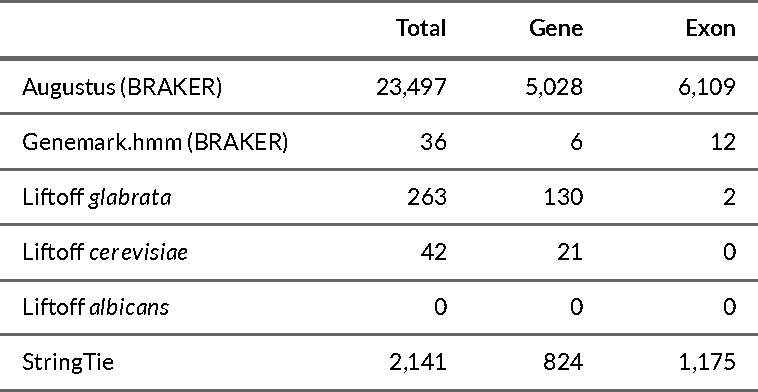
\includegraphics[width = .75\linewidth,keepaspectratio]{figure/genecounttable.pdf}
\caption[Contributions from each annotation software]{{\bf Contributions from each annotation software.} Number of genes and exons added by each software }
\label{tab:genecounttable}
\end{table}


\subsection{Data Availability}
\label{sec:methods}

All sequence data are available in the Sequence Read Archive, under BioProject PRJNA686979. This Whole Genome Shotgun project has been deposited at DDBJ/ENA/GenBank under the accession JAEVGP000000000. The version described in this here is version JAEVGP010000000. Code used for analysis is available at https://github.com/timplab/nivar.
